\documentclass{standalone}
\usepackage{tikz}
\usetikzlibrary{calc}
\usetikzlibrary{3d}
\usetikzlibrary{automata, positioning, arrows}
\tikzstyle{inarrow}=[->, >=stealth, shorten >=.03cm,line width=0.5]
\tikzstyle{outarrow}=[<-, >=stealth, shorten <=.03cm,line width=1.5]
\begin{document}
\rotatebox{0}{
\scalebox{1}{

    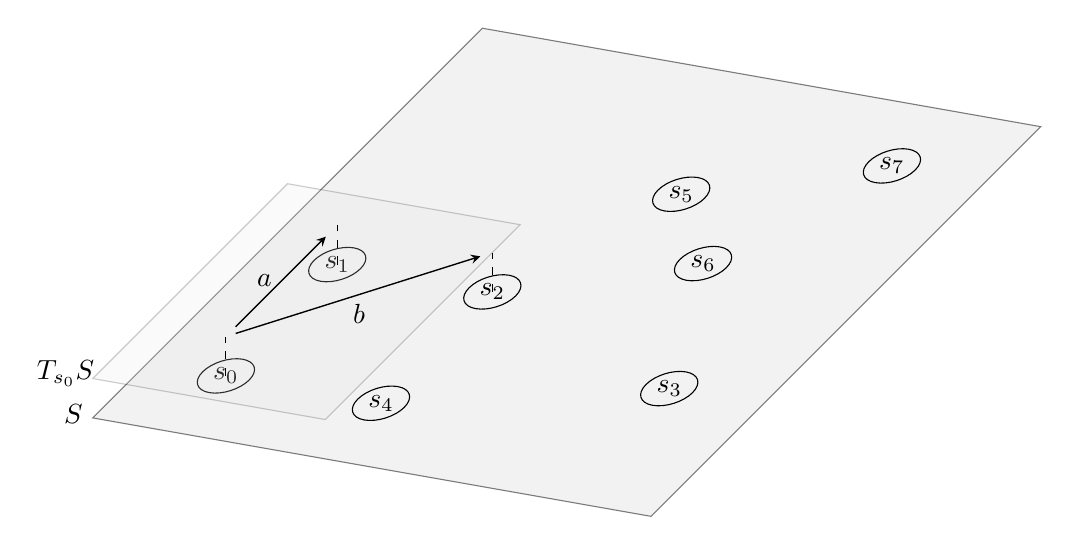
\begin{tikzpicture}[x={({cos(-10)*1cm},{sin(-10)*1cm})},y={({cos(45)*1cm},{sin(45)*1cm})},z={(0,1cm)}]
        % \coordinate (O) at (0, 0, 0);
        %     \draw[-latex] (O) -- +(1, 0,  0) node [right] {$x$};
        %     \draw[-latex] (O) -- +(0,  1, 0) node [left] {$y$};
        %     \draw[-latex] (O) -- +(0,  0, 1) node [above] {$z$};
        \begin{scope}[canvas is xy plane at z=0]
            \draw[fill=gray!20, opacity=0.5] (-1,-1) rectangle (6.2,6);
            \node (0) at (0,0) {$s_0$};
                \draw (0,0) circle (0.3cm);
            \node (1) at (0,2) {$s_1$};
                \draw (0,2) circle (0.3cm);
            \node (2) at (2,2) {$s_2$};
                \draw (2,2) circle (0.3cm);
            \node (3) at (5,1) {$s_3$};
                \draw (5,1) circle (0.3cm);
            \node (4) at (2,0) {$s_4$};
                \draw (2,0) circle (0.3cm);
            \node (5) at (3,4) {$s_5$};
                \draw (3,4) circle (0.3cm);
            \node (6) at (4,3) {$s_6$};
                \draw (4,3) circle (0.3cm);
            \node (7) at (5,5) {$s_7$};
                \draw (5,5) circle (0.3cm);
            
            \node (l) at (-1.25,-1) {$S$};
        \end{scope}
        
        \begin{scope}[canvas is xy plane at z=0.5]
            \draw[fill=gray!20, opacity=0.2] (-1,-1) rectangle (2,2.5);        
            \node (0) at (0,0) {};
            \node (1) at (0,2) {};
            \node (2) at (2,2) {};
            \node (3) at (5,1) {};
            \node (4) at (2,0) {};
            \node (5) at (3,4) {};
            \node (6) at (4,3) {};
            \node (7) at (5,5) {};
            \draw[inarrow] 
                (0) edge[left] node{$a$} (1)
                (0) edge[below] node{$b$} (2);

            \node (l) at (-1.35,-1) {$T_{s_0}S$};
        \end{scope}

        \draw[dashed] (0,0,0) -- (0,0,0.5);
        \draw[dashed] (0,2,0) -- (0,2,0.5);
        \draw[dashed] (2,2,0) -- (2,2,0.5);
        
\end{tikzpicture}}}
\end{document}